\documentclass[11pt]{article}

% ------------------------------------------------
% Packages
% ------------------------------------------------
\usepackage[a4paper,margin=2.5cm]{geometry}
\usepackage{amsmath,amssymb}
\usepackage{tikz}
\usetikzlibrary{arrows.meta,positioning,bending}

% ------------------------------------------------
% Document
% ------------------------------------------------
\begin{document}

%==================================================
% Paste the TikZ figure here
%==================================================

\begin{figure}[t]
\centering

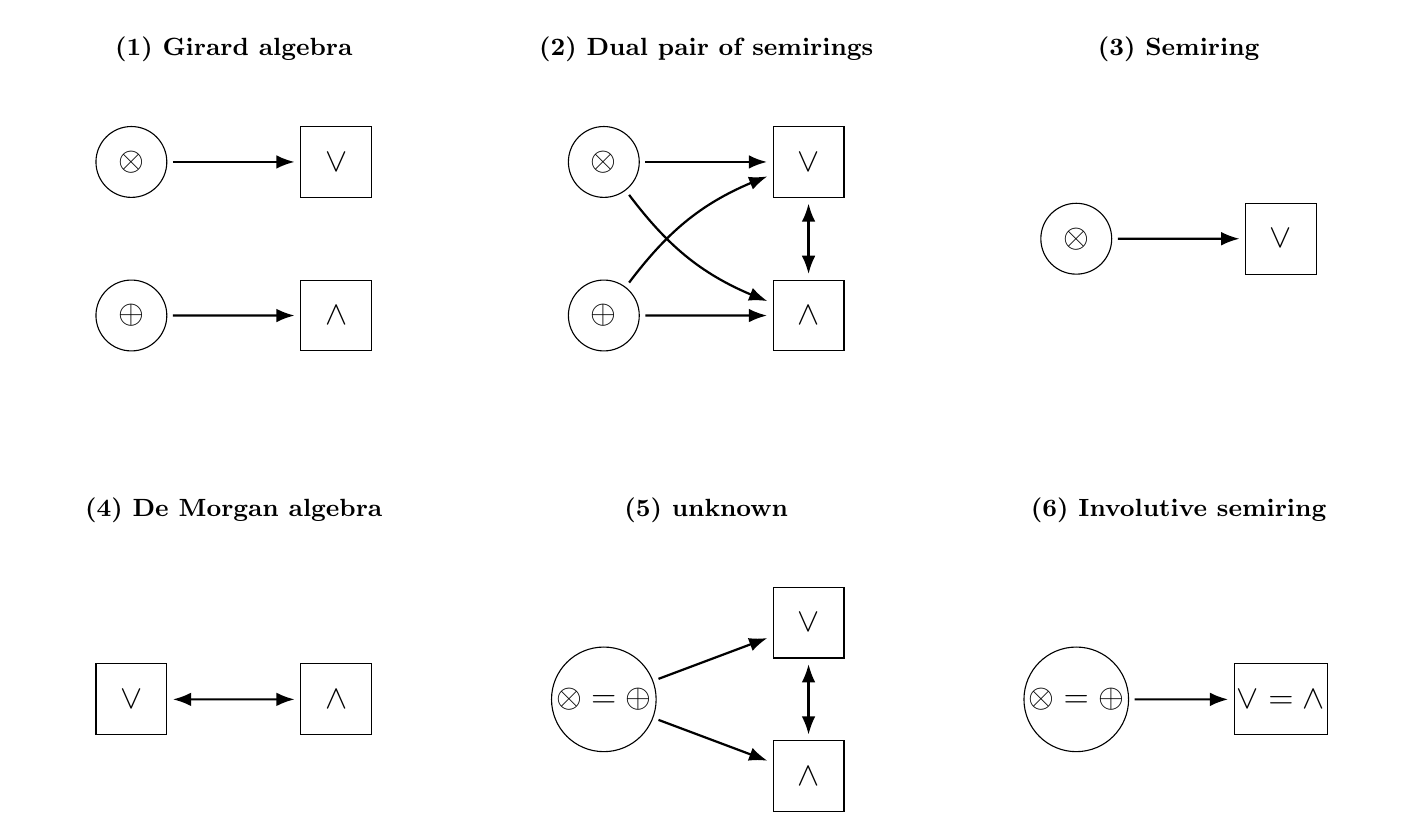
\begin{tikzpicture}[
    yscale=1.3,
    >=Latex,
    relation/.style={
        ->,
        thick,
        shorten >=2pt,
        shorten <=2pt
    },
    duality/.style={
        <->,
        thick,
        shorten >=2pt,
        shorten <=2pt
    },
    squareop/.style={
        draw,
        rectangle,
        minimum size=9mm,
        inner sep=1pt,
        font=\large
    },
    circleop/.style={
        draw,
        circle,
        minimum size=9mm,
        inner sep=1pt,
        font=\large
    },
    paneltitle/.style={
        font=\small\bfseries,
        align=center,
        text width=5cm
    }
]

% ============================================================
% Row 1
% ============================================================

% ------------------------------------------------------------
% 1. Polar semiring
% ------------------------------------------------------------
\begin{scope}[shift={(0,0)}]
    \node[paneltitle] at (2,1.1)
        {(1) Girard algebra};

    \node[circleop] (ps-tensor) at (0.7,0) {$\otimes$};
    \node[squareop] (ps-join)   at (3.3,0) {$\vee$};

    \node[circleop] (ps-plus)   at (0.7,-1.5) {$\oplus$};
    \node[squareop] (ps-meet)   at (3.3,-1.5) {$\wedge$};

    \draw[relation] (ps-tensor) -- (ps-join);
    \draw[relation] (ps-plus)   -- (ps-meet);
\end{scope}


% ------------------------------------------------------------
% 2. Dual pair of semirings
% ------------------------------------------------------------
\begin{scope}[shift={(6,0)}]
    \node[paneltitle] at (2,1.1)
        {(2) Dual pair of semirings};

    \node[circleop] (dp-tensor) at (0.7,0) {$\otimes$};
    \node[squareop] (dp-join)   at (3.3,0) {$\vee$};

    \node[circleop] (dp-plus)   at (0.7,-1.5) {$\oplus$};
    \node[squareop] (dp-meet)   at (3.3,-1.5) {$\wedge$};

    % Semiring distributivities
    \draw[relation] (dp-tensor) -- (dp-join);
    \draw[relation] (dp-plus)   -- (dp-meet);

    % Cross distributivities
    \draw[relation]
        (dp-tensor) to[bend right=15] (dp-meet);

    \draw[relation]
        (dp-plus) to[bend left=15] (dp-join);

    % Join--meet duality
    \draw[duality]
        (dp-join) -- (dp-meet);
\end{scope}


% ------------------------------------------------------------
% 3. Involutive semiring
% ------------------------------------------------------------
\begin{scope}[shift={(12,0)}]
    \node[paneltitle] at (2,1.1)
        {(3) Semiring};

    \node[circleop] (is-tensor) at (0.7,-0.75) {$\otimes$};
    \node[squareop] (is-join)   at (3.3,-0.75) {$\vee$};

    \draw[relation] (is-tensor) -- (is-join);
\end{scope}


% ============================================================
% Row 2
% ============================================================

% ------------------------------------------------------------
% 4. De Morgan algebra
% ------------------------------------------------------------
\begin{scope}[shift={(0,-4.5)}]
    \node[paneltitle] at (2,1.1)
        {(4) De Morgan algebra};

    \node[squareop] (dm-join) at (0.7,-0.75) {$\vee$};
    \node[squareop] (dm-meet) at (3.3,-0.75) {$\wedge$};

    \draw[duality] (dm-join) -- (dm-meet);
\end{scope}


% ------------------------------------------------------------
% 5. Three-operator structure
% ------------------------------------------------------------
\begin{scope}[shift={(6,-4.5)}]
    \node[paneltitle] at (2,1.1)
        {(5) unknown};

    % \node[circleop] (to-tensor) at (0.7,-0.75) {$\otimes$};
    \node[circleop] (to-tensor) at (0.7,-0.75){$\otimes=\oplus$};
    \node[squareop] (to-join)   at (3.3,0) {$\vee$};
    \node[squareop] (to-meet)   at (3.3,-1.5) {$\wedge$};

    \draw[relation] (to-tensor) -- (to-join);
    \draw[relation] (to-tensor) -- (to-meet);

    \draw[duality] (to-join) -- (to-meet);
\end{scope}


% ------------------------------------------------------------
% 6. Blank
% ------------------------------------------------------------
% ------------------------------------------------------------
% 6. Degenerate involutive semiring
% ------------------------------------------------------------
\begin{scope}[shift={(12,-4.5)}]
    \node[paneltitle] at (2,1.1)
        {(6) Involutive semiring};

    \node[circleop] (dis-tensor-plus) at (0.7,-0.75)
        {$\otimes=\oplus$};

    \node[squareop] (dis-join-meet) at (3.3,-0.75)
        {$\vee=\wedge$};

    \draw[relation]
        (dis-tensor-plus) -- (dis-join-meet);
\end{scope}

\end{tikzpicture}

\caption{Distribution profile of some algebras.}
\label{fig:algebraic-structure-comparison}
\end{figure}


\end{document}